% Created 2020-04-09 Thu 22:32
% Intended LaTeX compiler: pdflatex
\documentclass[11pt]{article}
\usepackage[utf8x]{inputenc}
\usepackage[T1]{fontenc}
\usepackage{graphicx}
\usepackage{grffile}
\usepackage{longtable}
\usepackage{wrapfig}
\usepackage{rotating}
\usepackage[normalem]{ulem}
\usepackage{amsmath}
\usepackage{textcomp}
\usepackage{amssymb}
\usepackage{capt-of}
\usepackage{hyperref}
\usepackage{unicode-math}
\author{Gianluca Scarpellini (gianluca@scarpellini.dev)}
\date{\today}
\title{Project 3 - Deep reinforcement learning - Collaboration and competition}
\hypersetup{
 pdfauthor={Gianluca Scarpellini (gianluca@scarpellini.dev)},
 pdftitle={Project 3 - Deep reinforcement learning - Collaboration and competition},
 pdfkeywords={},
 pdfsubject={},
 pdfcreator={Emacs 26.3 (Org mode 9.3.6)}, 
 pdflang={English}}
\begin{document}

\maketitle
\tableofcontents


\section{Introduction}
\label{sec:orgcfa22a6}
Deep Reinforcement Learning is today becoming a relevant field of research. The
current work aims to evaluate the ability of value-based methods of solving a
simple task in a constrained environment. In particular, we implemented Deep DPG
algorithm as presented during Udacity "Deep Reinforcement Learning" as well as
in the original paper for 2 competitive agents. We describe the environment in
section \ref{sec:org5ff204a}. A more in depth explanation of the approach is
presented in section \ref{sec:orgcd4bf78}. In section \ref{sec:org679590f} we comment the
results obtained with the algorithm. Finally, we take our conclusions in section
\ref{sec:org344ed33}.


\section{Environment and task}
\label{sec:org5ff204a}
The presented project is developed in order to solve the "Tennis" environment
with 2 agents in competition. The tasks consists in throwing the ball to
opposing competitor field. The reward is +0.1 for each right hit and a reward
of -0.01 for the wrong ones. The agents goal is to keep the ball in play as long
as possible. The observation space consists of 24 variables (position and
velocity of ball and racket). The action space is continuous and consists of a
vector of 2 continuous value corresponding to left-right movement and jump. The
task is episodic. The environment is considered solved if an average score of at
least \textbf{0.5} is maintained for 100 epochs.

\section{Algorithm and Implementation}
\label{sec:orgcd4bf78}
\begin{figure}[htbp]
\centering
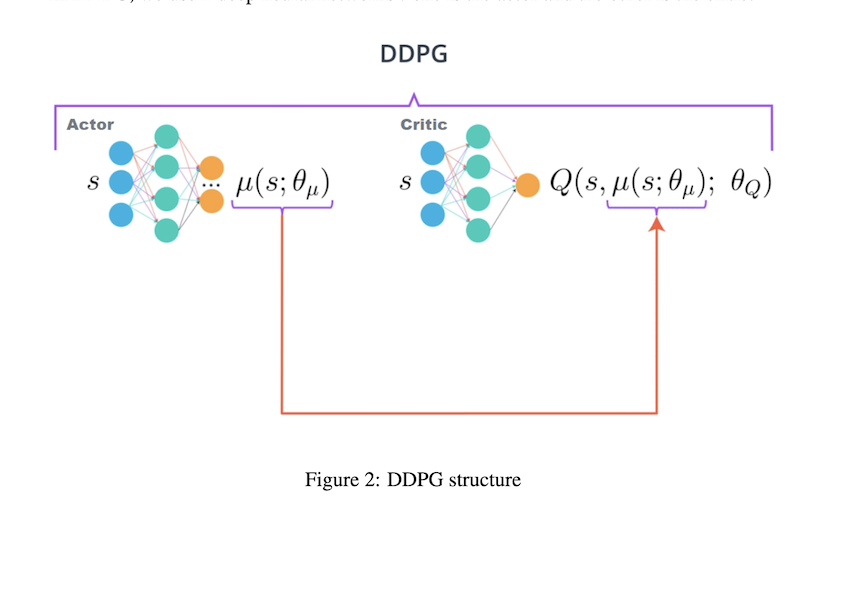
\includegraphics[width=.9\linewidth]{../contents/agentcritic.png}
\caption{\label{fig:orgb8e6bfa}Actor-critic approach}
\end{figure}

We used an actor-critic approach to solve the environment. Actor-critic methods
merges the idea of \textbf{policy-based} and \textbf{temporal-differences} in order to
mitigate their issues both in variance and bias. DDPG exploits 2 different
function approximators (such as neural networks, CNN, \ldots{}). The policy produces
by the actor is \textbf{deterministic}: the action per state is the optimal one. The
critic evaluates the deterministic policy and updates its parameters using
TD-error. The \textbf{deterministic policy gradient algorithm} is employed to update
the actor weights following equation in figure \ref{fig:org2db05e2}.


\begin{figure}[htbp]
\centering
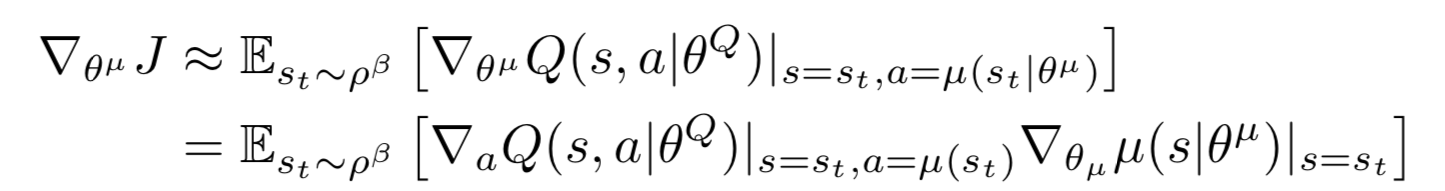
\includegraphics[width=.9\linewidth]{../contents/dpg.png}
\caption{\label{fig:org2db05e2}DPG equation}
\end{figure}

\subsection{Improvements}
\label{sec:org2a29a16}
We employed a few improvements proposed in the original DDPG article in order to
stabilize training.

\begin{itemize}
\item \textbf{Experience Replay}: The experience replay was originally proposed for Deep
Q-learning approach. It employs a buffer of finite size in order to sample
randomly from the state-action-rewards tuple space. Independent mini-batches
favor a more stable training. The states of both agents are pushed in the same
buffer for more stability.
\item \textbf{Soft updates}: In DDPG the target networks are updated using a \textbf{soft copy} of
the old weights. The result is a more smooth updating of neural networks
parameters.
\item \textbf{Parallelism}: We adapt DDPG in order to exploit a multi-agent
environment. The behavior of the algorithm is the same; the experience buffer
and the updates benefit from the high independence of the experiences coming
from different parallel agent.
\end{itemize}

\subsection{Hyperparameters}
\label{sec:org3506835}
For the experiment we used the following hyperparameters:

\begin{center}
\begin{tabular}{lr}
Hyperparameter & Value\\
\hline
Replay buffer size & 1e6\\
Batch size & 1024\\
\(\gamma\) & 0.99\\
\(\tau\) & 1e-3\\
Actor lr & 1e-4\\
Critic lr & 1e-3\\
Update every & 20\\
Update times & 10\\
Episodes & 5000\\
\hline
\end{tabular}
\end{center}


\section{Results}
\label{sec:org679590f}
In figure \ref{fig:orgd6d4ae0} it's presented the algorithm result per episode. In
particular, we were able to solve the environment in less then 50 epochs. The
scores kept growing until an optimal maximum of 2.0, probably due to limited
time play per episode. The learning was flat until when it started reaching a
local maximum. There was some noise in the precess, probably due the multi-agent
environment. Different approaches and improvements are discussed in section
\ref{sec:org344ed33}.

\begin{figure}[htbp]
\centering
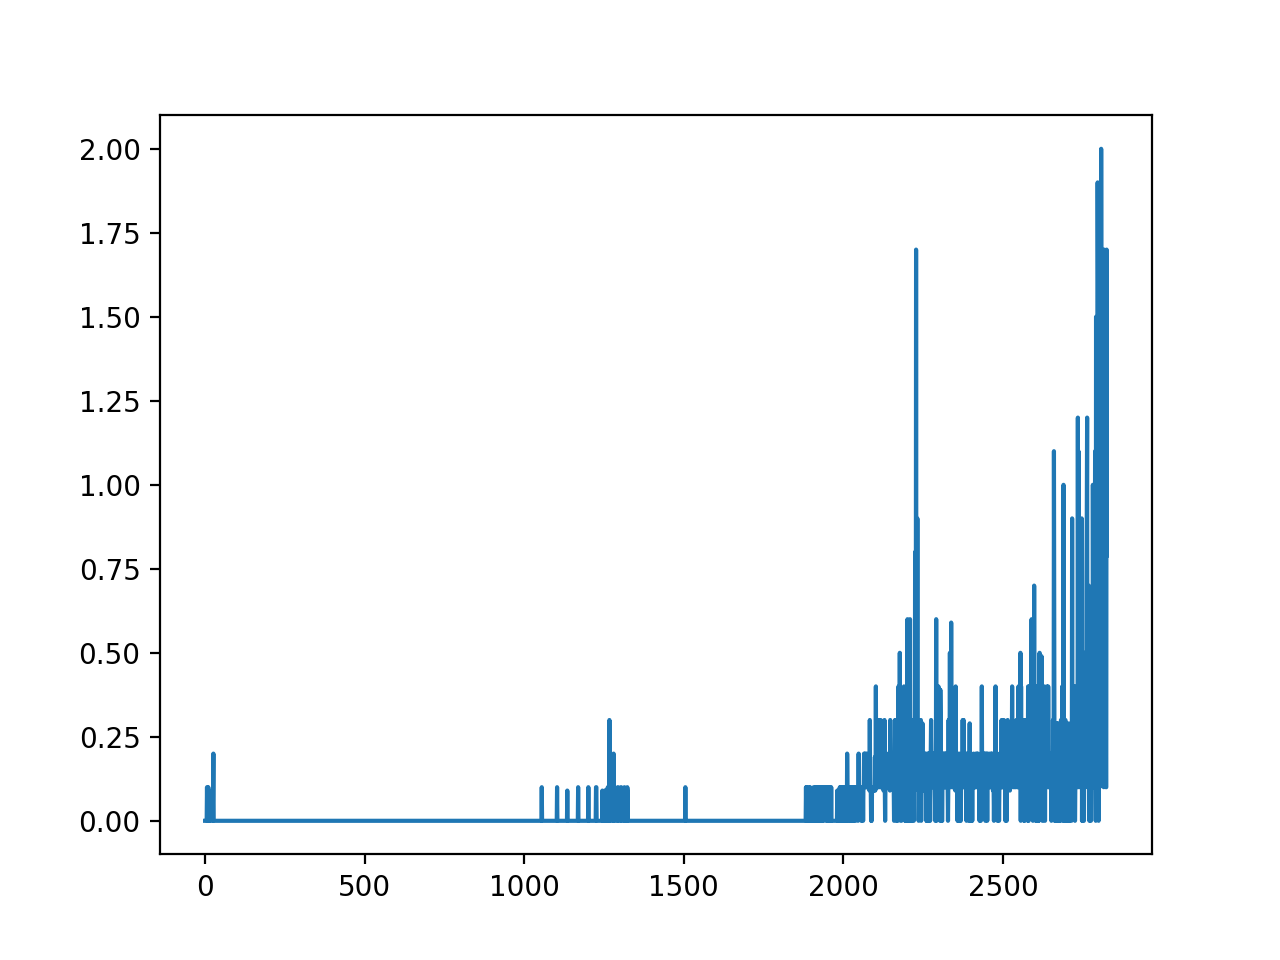
\includegraphics[width=.9\linewidth]{../contents/solved.png}
\caption{\label{fig:orgd6d4ae0}Learning scores per epoch}
\end{figure}

\section{Conclusion and further}
\label{sec:org344ed33}
We developed a pipeline in order to solve `tennis` environment with Deep
Reinforcement Learning. In particular, we implemented \textbf{Deep Deterministic Policy
Gradient} following the paper specification. DDPG is an off-policy actor-critic
algorithm which has proven stability and optimal results in multiple tasks. We
believe better results in terms of training speed could be achievable using more
advances algorithms like PPO for continuous action. As a matter of fact, PPO
could better benefit from the parallelism offered by the environment. We can
improve the experience sampling by using a priority based sampling technique to
help the agent with the exploration/exploitation problem. More advance solutions
could involve D4PG algorithm or Hindsight Experience replay. 
\end{document}